% BEGIN TEMPLATE
\documentclass{article}
\usepackage{graphicx}
\usepackage{hyperref} 
\usepackage{xcolor}
\usepackage{nameref}
\usepackage{listings}
\usepackage{float}
\usepackage[title]{appendix}
\graphicspath{ {../../images/} }
\bibliographystyle{acm}
% CHANGE THESE
\newcommand{\courseListing}{CSCI 8920}
\newcommand{\courseName}{Fundamentals of Deep Learning}
\newcommand{\assignmentTitle}{Homework Assignment \#1}
\newcommand{\assignmentSubtitle}{Dataset Processing Functions}
\usepackage{geometry}
\geometry{margin=1in}

\hypersetup{
    colorlinks,
    linkcolor={red!50!black},
    citecolor={blue!50!black},
    urlcolor={blue!80!black}
}
\urlstyle{same}
\definecolor{codegreen}{rgb}{0,0.6,0}
\definecolor{codegray}{rgb}{0.5,0.5,0.5}
\definecolor{codepurple}{rgb}{0.58,0,0.82}
\lstdefinestyle{mystyle}{
    commentstyle=\color{codegreen},
    keywordstyle=\color{magenta},
    numberstyle=\tiny\color{codegray},
    stringstyle=\color{codepurple},
    basicstyle=\ttfamily\footnotesize,
    breakatwhitespace=false,         
    breaklines=true,                 
    captionpos=b,                    
    keepspaces=true,                 
    numbers=left,                    
    numbersep=5pt,                  
    showspaces=false,                
    showstringspaces=false,
    showtabs=false,                  
    tabsize=2
}

\lstset{style=mystyle}

\begin{document}
  \begin{center}
  
\includegraphics[scale=0.15]{UNO-Logo-Color.png}
  \\[0.3in]
  \textbf{\courseListing{}}\\
  \courseName{}
  \\[0.75in]
  \textbf{\assignmentTitle{}}\\
  \assignmentSubtitle{}
  \\[0.75in]
  \textbf{Patrick Davlin}
  \\[0.75in]
  \textbf{Computer Science Department}\\
  \textbf{Peter Kiewit Institute}\\
  \textbf{University of Nebraska}
  \\[0.75in]
  \textbf{Spring 2021}
  \\[0.3in]
  
\includegraphics[scale=0.075]{UNO-Icon-Color.png}
  \newpage
\end{center}
  \graphicspath{{./images/}}
% END TEMPLATE
\section{Introduction}
A critical component of any deep learning project is developing an intimate understanding of the data upon which that project will act.
One thing learned last semester in the Advanced Applications class is that there is no model of any sophistication that can be run on random data; every project is unique and requires careful selection and assembly for training data.
Speaking generally, models are developed around two different sets of data-- \textit{training} and \textit{testing} (or \textit{validation}) data.
In this assignment, several different methods of organizing training and validation data were implemented for comparison:
\begin{itemize}
    \item \textbf{Holdout}: splitting a dataset directly into training/validation sets (generally, 70/30, respectively);
    \item \textbf{K-Fold Cross-Validation}: dividing a dataset into several groups, then rotating through each single group as the validation data, while remaining groups are training data;
    \item \textbf{Bootstrapping}: generating datasets of a set length randomly, with replacement; and,
    \item \textbf{Batch generation}: generating datasets of a set length sequentially, using data from the start of the dataset to "fill in" if the end of the dataset is reached.
\end{itemize}


\section{Project Setup} \label{setup}
At the end of the CSCI 8110 course, I was able to obtain a new Nvidia GTX 3080 card.
At the time, the CUDA 8 architecture on the card was not well-supported, so assignments needed to be done on a combination of personal hardware (Windows) and online applications (Paperspace Gradient or Google Colab).
Months later, Tensorflow has substantially better support for newer cards.
On a full re-install of Windows, Tensorflow was up and running in under an hour without any trouble.
As such, this assignment was done entirely on a local machine using the following specific packages:
\begin{itemize}
    \item Python 3.8.6 
    \item Tensorflow 2.4.1
    \item Matplotlib 3.3.4
\end{itemize}.

\section{Implementation} \label{impl}
\textit{Note: this section discusses sections of code; the entire project can be found in the \nameref{codelist}}.
\\\\
The first task for the assignment was to load and output CIFAR10 data:
\begin{lstlisting}[language=Python]
# Load CIFAR10 data
(cifar10_data, _), (_, _) = cifar10.load_data()
cifar10_data = cifar10_data / 255

# Display sample images
plot_cifar_img(cifar10_data)
\end{lstlisting}
To confirm, the resulting images are below:

\begin{figure}[H]
    \centering
    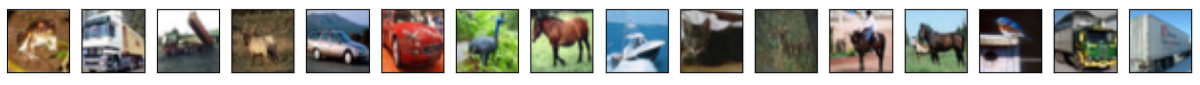
\includegraphics[width=6in]{csci-8920/hw-1/images/8920-hw-1-cropped.png}
    \caption{CIFAR-10 images}
    \label{fig:data}
\end{figure}

Implementing the first three methods (Holdout, K-Fold, and Bootstrapping) was a fairly straightforward exercise.
Being listed first, and being the most straightforward, the holdout function was implemented as a simple way to create a pre-defined split of the provided data:
\begin{lstlisting}[language=Python]
def holdout(data_in,training_pct=0.7):
  num_records_in_training_set=int(len(data_in) * training_pct)
  np.random.shuffle(data_in)
  training_data = data_in[0:num_records_in_training_set]
  validation_data = data_in[num_records_in_training_set:]
  return training_data, validation_data
\end{lstlisting}

For a dataset with 50,000 entries, like the CIFAR-10 data, the split comes out to 35,000 training images and 15,000 testing images.


\section{Results \& Observations} \label{observations}
\section{Conclusions}
Having extensively used Keras models in CSCI 8110, without thinking of the ways that datasets are used in training and validating those models, made this assignment much more valuable.
Oftentimes in that class, models I implemented were "thrown" together without much of an eye toward the quality or organization of data being used as a basis upon which the model would operate.

\newpage
\begin{appendices}
\section{Complete Program Output}
\lstinputlisting{hw-1.py}
\section{Complete Code Listing} \label{codelist}
\lstinputlisting[language=Python]{hw-1.py}
\end{appendices}
\end{document}